\documentclass[fleqn]{article}
\usepackage{amsmath}
\usepackage[dvips]{graphicx}
\bibliographystyle{plain}
%__________________________________SHOCKTUBE 1 level
\begin{document}

\section*{\center Shock Tube}
\subsection*{\underline{Problem Description}}
The shock tube problem is a standard 1D compressible flow problem that has been used by many as a
validation test case \cite{laney, sod, toro}.  At time $t=0$ the computational domain is divided
into two separate regions of space by a diaphram, with each region at a different density and
pressure.  The separated regions are at rest with a uniform temperature $=300K$.  The initial
pressure ratio is $\frac{P_R}{P_L}  = 10$ and density ratio is $\frac{\rho_R}{\rho_L} = 0.1$  The
diaphram is instantly removed and a traveling shockwave, discontinutity and expansion fan form.  The
expansion fan moves towards the left while the shockwave and contact discontinutity move to the
right.  This problem tests the algorithm's ability to capture steep gradients and solve Eulers equations. 
 
\subsection*{\underline{Simulation Specifics}}
\begin{description} 
\item [Component used:] \hfill ICE
\item [Input file name:] \hfill shocktube.ups
\item [Command used to run input file:]\hfill sus shocktube.ups
\item [Postprocessing command:]\hfill \\
inputs/UintahRelease/ICE/plot\_shockTube\_1L shockTube.uda

\item [Simulation Domain:]\hfill    1 x .01 x .01 m
\item [Cell Spacing:]\hfill \\ 
0.1 x 10 x 10 mm (Level 0)

\item [Example Runtimes:] \hfill \\
 2 minutes   (1 processor, 2.4 GHz Xeon)

\item [Physical time simulated:] \hfill 0.005 sec.

\end{description}

\section*{\underline{Results}}
Figure \ref{results} shows a comparison of the exact versus simulated results at time $t = 5msec$.
\begin{figure}
\includegraphics[scale=.85]{figures/shockTube.ps}
\caption{Shock tube results at time $t = 5msec$}
\label{results}
\end{figure}
\newpage

%__________________________________SHOCKTUBE AMR

\section*{\center Shock Tube with AMR}
 
\subsection*{\underline{Simulation Specifics}}
\begin{description} 
\item [Component used:] \hfill ICE
\item [Input file name:] \hfill shocktube\_AMR.ups
\item [Command used to run input file:]\hfill sus shocktube\_AMR.ups
\item [Postprocessing command:]\hfill \\
inputs/UintahRelease/ICE/plot\_shockTube\_AMR shockTube\_AMR.uda

\item [Simulation Domain:]\hfill    1 x .01 x .01 m
\item [Cell Spacing:]\hfill \\ 
0.1 x 10 x 10 mm (Level 0)
0.025 x 10 x10 mm (Level 1)
0.00625 x10 x10 mm (Level 2)


\item [Example Runtimes:] \hfill \\
 2ish minutes   (1 processor, 2.4 GHz Xeon)

\item [Physical time simulated:] \hfill 0.005 sec.

\end{description}

\section*{\underline{Results}}
Figure \ref{results} shows a comparison of the exact versus simulated results at time $t = 5msec$.
\begin{figure}
\includegraphics[scale=.85]{figures/shockTube_AMR.ps}
\caption{Shock tube results at time $t = 5msec$}
\label{results}
\end{figure}
\newpage



\bibliography{../references}

\end{document}
